\chapter{Fringing Effects in MIRI}\label{ch:fringe}
Understanding optical and instrumental effects is critical for creating accurate simulated observations and for characterizing systematics. 
These systematics and uncertainties in turn impact the potential science results from any instrument by biasing measurements, reducing the signal to noise ratio of measurements or by injecting non-physical signals and correlations.
The aim of this chapter is to examine fringing in the MIRI detectors and how this effect is modeled in the instrumental simulator (MIRISIM). 
We will examine the current status of fringe modeling and correction before discussing the modifications made to the MIRI instrumental simulator in order to model point-source fringing effects.

In order to quantify the effect of fringing on a spectrum, we examine the effect of fringing on a cross correlation between the extracted spectrum from the instrument and a known template. 
This provides a measure of the extent to which the signal has been degraded.
In addition we examine the impact of this on the science case of molecular mapping, where cross correlations between a cube of IFU data and a molecular spectral template are used to identify the presence of a given species in an observed object. 

\section{Fringing}
Thin film interference occurs when light is coherently reflected at the internal boundaries between two layers and interferes with the incident light.
This is the principle on which Fabry-P\'{e}rot interferometers function.
As we wish to determine the effect of fringing on the amplitude of the signal received by the detector as a function of wavelength, we are effectively interested in the transmittance of a series of Fabry--P\'{e}rot interferometers. 
Assuming an ideal plane-parallel optical cavity with a reflectance R at both boundaries, thickness D, and an angle $\theta$ at which the light enters the cavity, we can compute the transmittance as:
\begin{equation}\label{eqn:trans}
T_{c} = \frac{1}{1+\frac{4R}{\left(1-R\right)^{2}}\sin^{2}\left(\frac{\delta}{2}\right)}
\end{equation}
Where the phase $\delta$ at half a wavelength ($\phi = \pi$), with wavenumber $\sigma$ is:
\begin{equation}\label{eqn:phase}
\delta = 4\pi\sigma D \cos\theta - (\phi - \pi)
\end{equation}
Systems with a spacing on the order of micrometers to millimeters produces significant interference for infrared light \parencite{Lahuis2003}.

The detectors of the MRS consist of several layers, as shown in Fig. \ref{fig:layers}, with a characteristic thickness of tens of micron, which results in significant (10\%-30\%) `fringing' in a spectrally flat signal - visible in Fig. \ref{fig:flatfield}.
The geometric thicknesses of the detector layers are given in table \ref{tab:layers}.

While this is typical for infrared detectors such as those in the Spitzer Space Telescope \parencite{Lahuis2003} or in the Space Telescope Imaging Spectrograph on board HST \parencite{Malumuth2003}, the sensitivity and spectral resolution of the MRS increases the significance of this issue.
The MIRI consortium has stated that the error budget for all detector effects must be 3.3\% or less. 
Present fringing corrections result in a 5\% deviation from a photometrically accurate signal, and can introduce correlated noise which will degrade any measured spectrum.
Therefore it is critical to examine the impact of fringing on a signal, the parameters that influence the fringing strength and phase, and possible solutions for fringe correction. 
If all of the geometric and optical parameters were known, this would be sufficient to numerically solve for the fringing pattern within MIRI using eqn \ref{eqn:trans}. 
Unfortunately, uncertainties in the thickness in the detector layers, variations in the layer deposition thickness, and the uncertainty of transmittance and reflectance of the materials used at cryogenic temperatures prevents the implementation of such a numerical model.
Instead, we will turn to calibration data taken to empirically characterize the fringing pattern.

While a more complete treatment of proposed fringe correction can be found in \parencite{Argyriou2020} and \parencite{Lahuis2018}, this work will examine the implementation of fringing into the MIRI instrumental simulator and address the current state of fringe correction in the JWST Data Calibration Pipeline.
We will discuss the architecture and usage of MIRISIM, along with the modifications we have made in order to model point-source fringing.

\definecolor{lightgray}{HTML}{E0E0E0}
\definecolor{darkgray}{HTML}{383838}
\begin{figure}
	\centering
	\begin{scriptsize}
		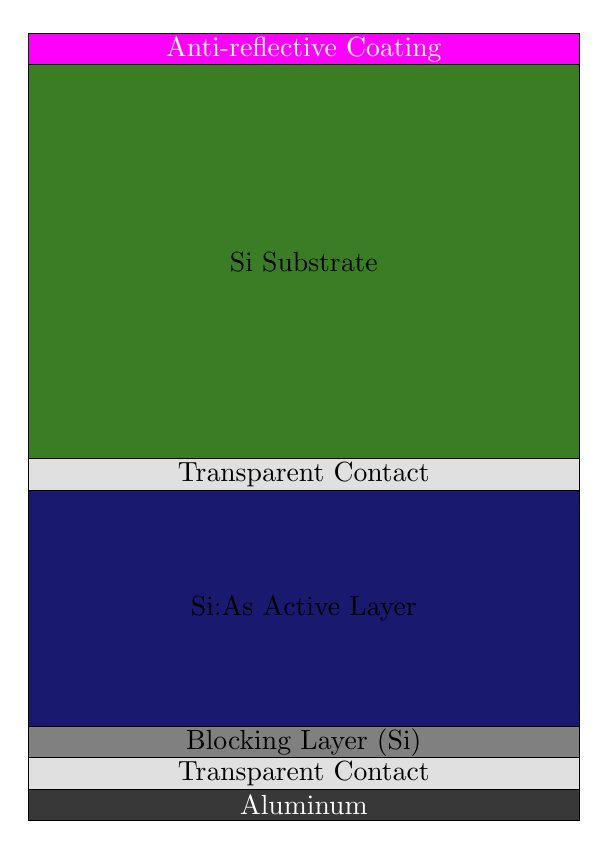
\begin{tikzpicture}
		\filldraw [fill=darkgray, draw=Black](0,0) rectangle (7,0.4) node [pos=0.5] {\textcolor{White}{Aluminum}};
		\filldraw [fill=lightgray, draw=Black](0,0.4) rectangle (7,0.8) node [pos=0.5] {Transparent Contact};
		\filldraw [fill=Gray, draw=Black](0,0.8) rectangle (7,1.2) node [pos=0.5] {Blocking Layer (Si)};
		\filldraw [fill=MidnightBlue, draw=Black](0,1.2) rectangle (7,4.2) node [pos=0.5] {Si:As Active Layer};
		\filldraw [fill=lightgray, draw=Black](0,4.2) rectangle (7,4.6) node [pos=0.5] {Transparent Contact};
		\filldraw [fill=OliveGreen, draw=Black](0,4.6) rectangle (7,9.6) node [pos=0.5] {Si Substrate};
		\filldraw [fill=Fuchsia, draw=Black](0,9.6) rectangle (7,10) node [pos=0.5] {\textcolor{White}{Anti-reflective Coating}};
		\end{tikzpicture}
	\end{scriptsize}
	\caption{Layers of the MIRI MRS detectors. Note that thicknesses are not to scale \parencite{MIRI7}.}
	\label{fig:layers}
\end{figure}
\begin{table}[h]
	\centering
	\begin{footnotesize}
	\begin{tabular}{llll}
		\toprule
		\textbf{Layer} & \textbf{Material} & \textbf{Depth [$\mu$m]} & \textbf{Comments}\\
		\midrule 
		Anti-Reflection Coating & ZnS & 0.66 & Optimized for $\lambda$ = 6$\mu$m.\\
		Substrate (raw wafer) & Si & 460 & Inactive layer.\\
		\multirow{2}{*}{Bottom Transparent contact} & \multirow{2}{*}{?} & \multirow{2}{*}{?} & Not transparent,\\&&& negative applied bias voltage.\\
		Active layer & Si:As & 35 & Photoelectric absorption layer.\\
		Blocking layer & Si & 4 & Inactive layer.\\
		\multirow{2}{*}{Top transparent contact} & \multirow{2}{*}{?} & \multirow{2}{*}{?} & Not transparent.\\&&& Positive applied bias voltage.\\
		\multirow{2}{*}{Pixel metalization} & \multirow{2}{*}{Al} & \multirow{2}{*}{semi-infinite} & Forms metallized electrical contact\\ &&&with top transparent layer.\\
		\bottomrule
	\end{tabular}
	\end{footnotesize}
	\caption{Detector layer compositions and mean geometric thicknesses.}
	\label{tab:layers}
\end{table}

\subsection{Current Status of Fringing Correction}
Three test campaigns have been run in order to characterize MIRI: the Flight Model (FM) in 2008-09, the Cryogenic Vacuum (CV) in 2015-16, and the Optical Telescope element/ Integrated Science (OTIS) tests in 2017. 
Fringing was a major subject of both the FM and CV campaigns
The first fringe model is fit to a spectrally flat, spatially extended source based on the FM test data.
This is used to derive a `fringe flat', and example of which is presented in \ref{fig:fringeflat}.
The extended source fringe flat is used both in MIRISIM to model the effect as well as in the JWST pipeline to correct for it.

This basic correction is insufficient to properly correct for fringing, and in the worst case can add additional fringing effects to the data. 
Therefore an additional iterative correction is used to attempt to remove fringing frequencies in Fourier space \parencite{Lahuis2003,Lahuis2018}.
Unfortunately, this can also remove real signals from the data.
\parencite{Argyriou2020} proposes a novel method for fringe correction based on modeling sources as a collection of point sources, leading to a sum of overlapping point source fringe patterns.
They show that this improves fringing correction to sub-percent levels, with mostly uncorrelated residuals.

Due to the dependence of fringing on the incident angle of the light, a single extended source model of fringing is insufficient to describe the full effect. 
In this work, we implement a more realistic fringing model based on point-source FM data and the concepts described in \parencite{Argyriou2018a}. 
Data at various points across the detector is used to apply a unique position dependent fringe flat.
We  will quantify how this changes the extracted spectra after processing in the JWST pipeline, and examine to what extent present correction methods can remove the point-source fringing.

%\parencite{VanderPlas2018}

% - FRINGING REQUIREMENTS FOR MIRI - context
% - sub percent residuals - is this true and if so how much does it impact real spectral %features?
% - What has been done so far - fitting, optical modelling
% - only for some channels
% - Might remove actual spectral features as well - justification for this work (especially re posn dependence)
% - need to reproduce plots from fringing white paper
% - explain why point sources are harder (angle => optical thickness => large phase shift)
% - 
%\cite{Lahuis2018} %MIRI MRS FM Fringing Analysis
\section{MIRISIM}

%MIRISIM in python
The MIRI instrument has been simulated in python as a program known - perhaps unsurprisingly - as MIRISIM \parencite{ref:mirisimdocs}. 
This program takes in an astronomical `scene' along with some configuration parameters to output a detector data product, similar to what will be produced by the actual instrument.
MIRISIM is relatively full-featured simulator, modeling the instrumental PSF, various noise sources and distortion maps, among other effects.
While MIRISIM is functional for all of the MIRI sub-instruments, this report will only deal with the Medium-Resolution Spectrometer (MRS) sub instrument, described in section \ref{sec:mrs}.
The objective of this section is to describe the implementation and testing of an updated optical model of the `fringing' effect - an optical effect caused by thin film interference from the multiple layers of the detector.
\subsection{Architecture}
While the full documentation for MIRISIM is available in \parencite{ref:mirisimdocs} and with python documentation in \parencite{Cossou2018}, in this section we will outline the procedure for generating a simulated detector image.
In particular, we will emphasize the parameter choices made in the setup for our simulations.

A MIRISIM simulation begins by setting up a \textbf{scene} using the \verb|skysim|. 
This represents the view that the telescope will have of some astrophysical system.
In general, a scene can be built from nearly anything: a fits file of an actual observation, models of galaxies and more. 
Built in are tools for producing simple point source and extended source objects.
An SED of arbitrary spectral resolution is then attached to the object from an external file, with units of micron for the wavelength and $\mu$Jy for the incident flux on the detector.
There are also built in tools for blackbody SEDs, and individual lines of arbitrary position and depth.
All of our SEDs are generated using petitRADTRANS, and attached as an external spectrum.
A background can be applied, representing both astrophysical emission sources as well as thermal emission from the telescope itself.
We chose not to include a background term, as background subtraction is using a simple model and image-from-image subtraction will result in an ideal correction.

For our observations, we only consider a single point source within the field of view.
While this is an oversimplification, particularly in the case of close in planets, it is not the purpose of this thesis to explore the procedures for extracting a companion spectrum in a contrast limited regime.
Instead, we assume that the spectral extraction will be adequate, though our simplification provides somewhat of a best case scenario.

The scene is then processed using a set of instrument and detector simulators \verb|obssim|, \verb|scasim| and \verb|specsim|.
These make use of the calibration data products (CDPs) in order to model optical distortions and detector effects.
The output of this simulation is a set of uncalibrated data files, similar to what will be produced with on-sky observations.
From the scene, an illumination model is produced. This transforms the on sky image using telescope and instrument optics in order to produce the intensity pattern incident on the detector itself.
As our observations make use only of the MRS, they are then processed using \verb|specsim|, which makes use of the \verb|pySpecSim| module.
This module is where most instrumental effects are applied, including detector sensitivities and fringing.
These are applied by multiplying the illumination model by the CDPs. 
The set of fringe CDPs covers each of the MRS sub-bands, and contains a fringe flat.
This is a 2D array of multiplicative factors used to apply the fringe pattern to the illumination model, an example of which is given in Fig \ref{fig:fringeflat}. 
Presently, these are derived from extended source CV data, CDP version 07.02.05.
Once detector effects are applied, and the incident flux is converted into DN counts, a detector image is produced and stored in a fits file.
A raw detector image for WISE 0855 is shown in Fig. \ref{fig:0855raw}

When running a simulation, the user must set the observation parameters.
This includes setting the instrument used (MRS), dither pattern, readout mode, and further MRS parameters.
Our parameter selections  are based on the parameters used in the JWST ERS and GTO proposals for our target objects, described in more detail in \ref{sec:obs} and summarized in table \ref{tab:obsparams}.
\begin{figure}[t]
	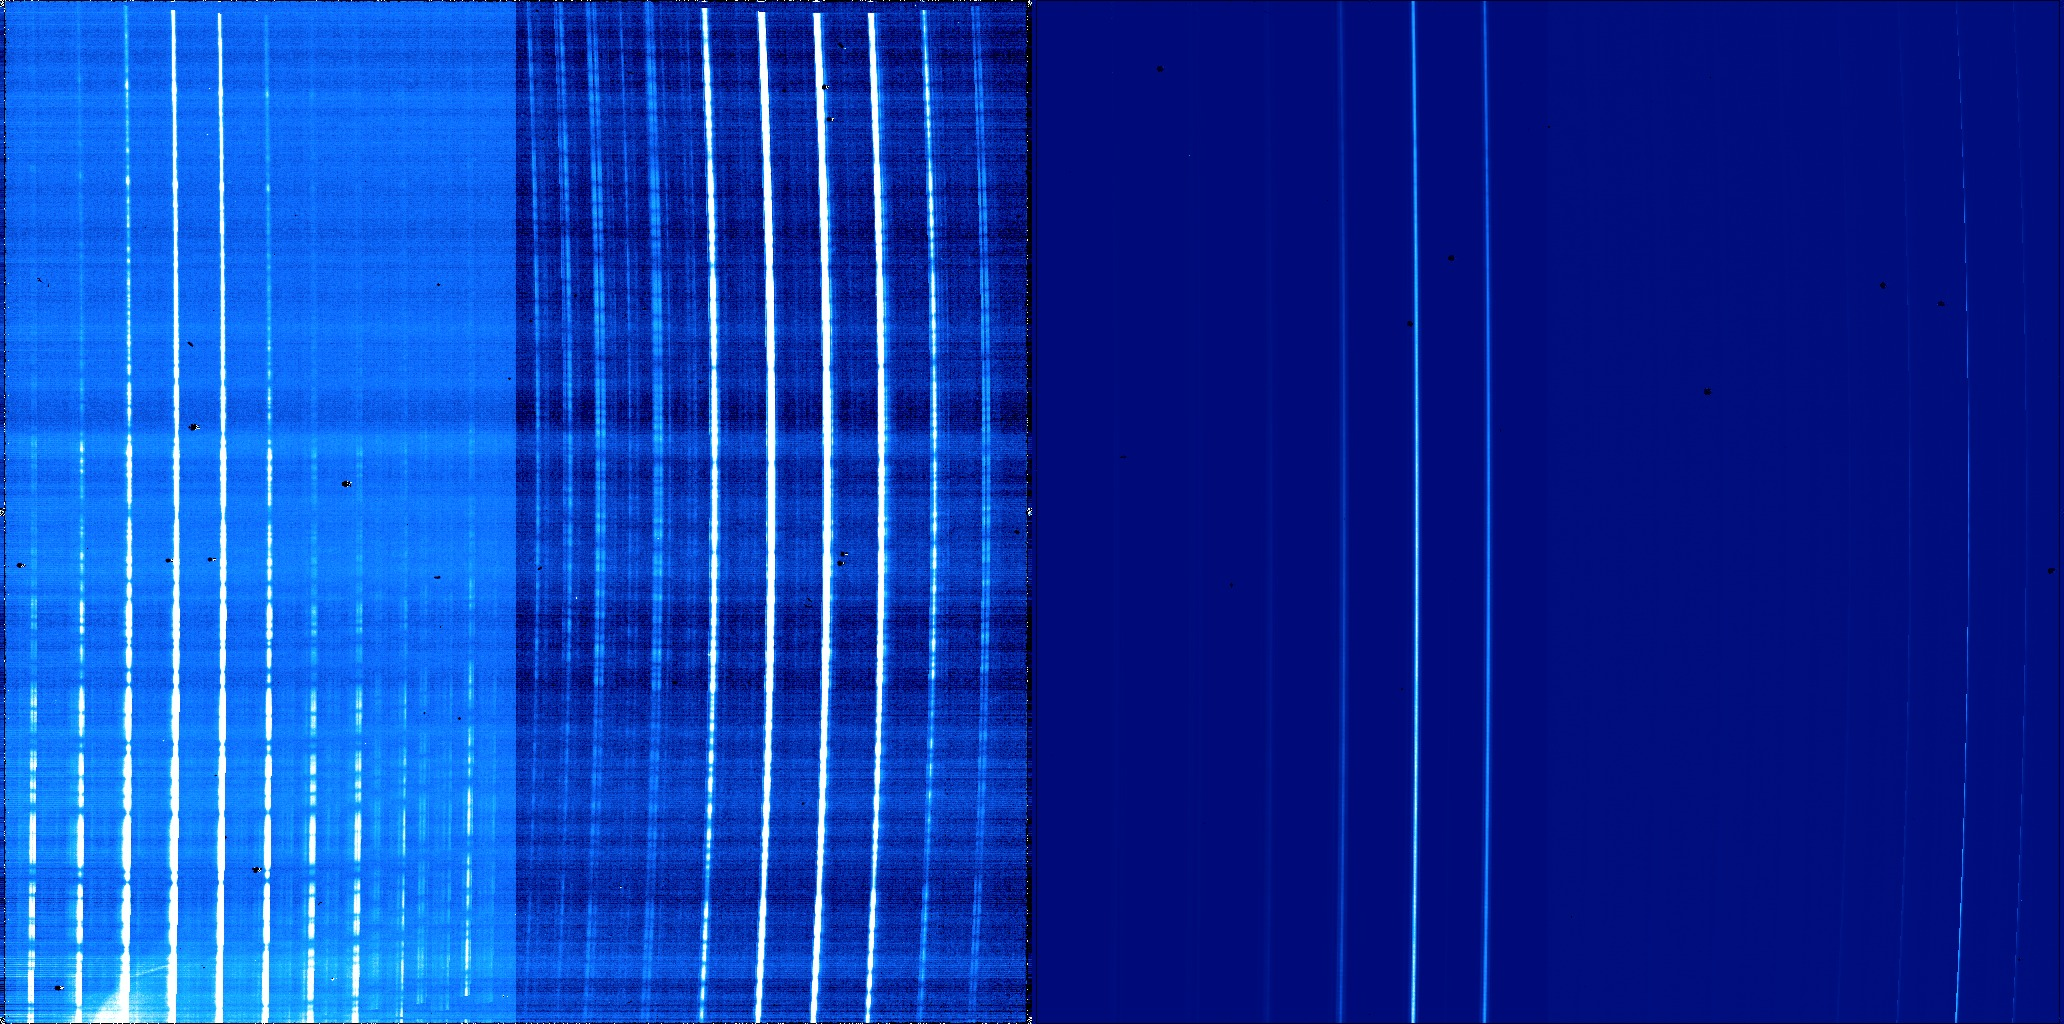
\includegraphics[width=\linewidth]{WISE0855_1234SHORT_RAW.jpg}
	\caption{\textbf{Right Panel:} Channel 1 (left) and Channel 2 (right). \textbf{Left Panel:} Channels 3 (right) and 4 (left). Observation of WISE 0855 using the SHORT disperser. Fringing has been disabled for this particular observation. The color scale is in sqrt(DN) to highlight faint features.}
	\label{fig:0855raw}
\end{figure}

\subsection{Data Products}
\begin{wrapfigure}{r}{5.5cm}
	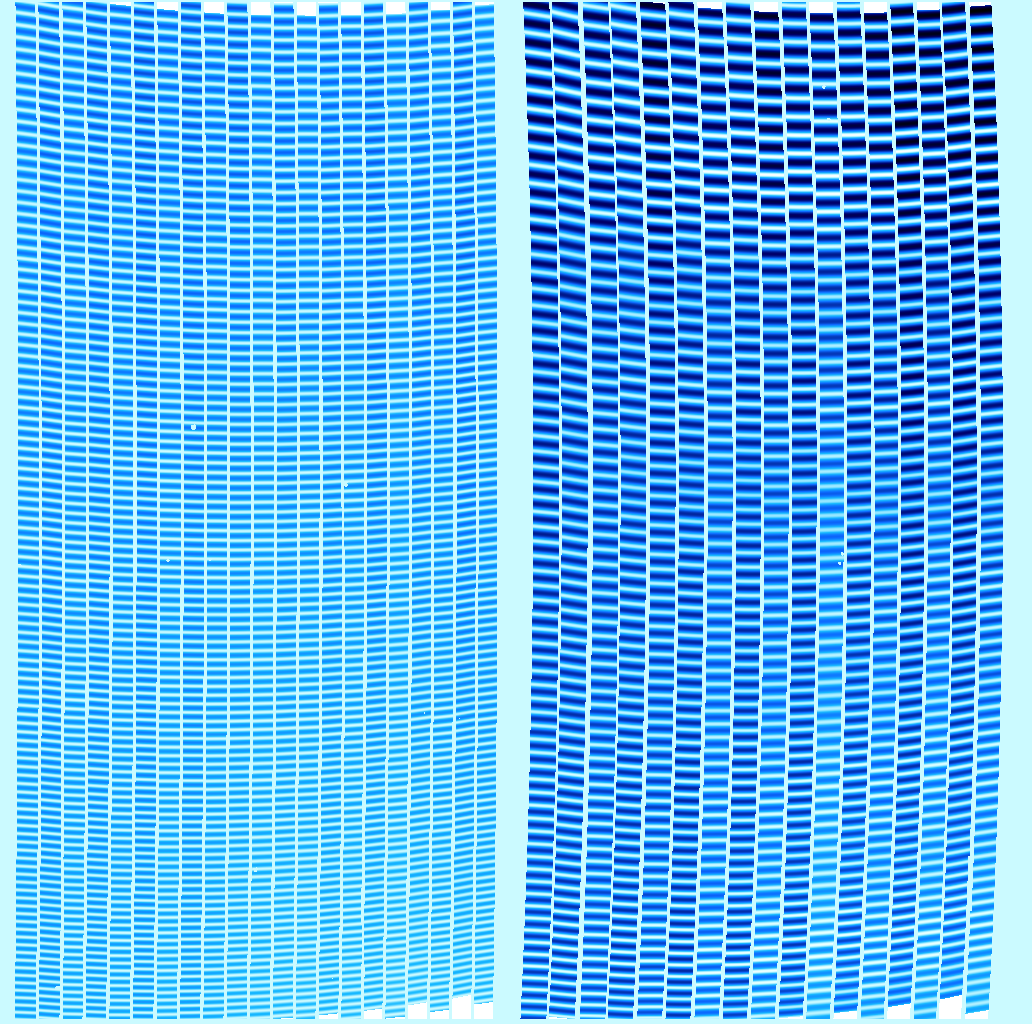
\includegraphics[width=5.5cm]{12SHORT_FRINGE_070200.png}
	\caption{Fringe flat derived from FM data for the SW detector, in the SHORT sub-band v07.02.00. Color scale is linear.}
	\label{fig:fringeflat}
\end{wrapfigure}
All of the CDP files are derived from test campaign data, and represent the best empirical knowledge of the instrument.
The primary CDPs of interest for this project are the photometric calibration data products and the fringe flats.
The PHOTOM files map the sensitivity of each detector pixel in order to represent the varying sensitivity of the detectors with wavelength. 
They convert from an incident flux to detector counts based on measured efficiencies.
Recently the PHOTOM files were modified from being divided into the illumination model to being multiplied in. 
This, along with other issues, has led to inconsistencies between the input flux and output of the JWST pipeline.
To best correct for this, we ensure that we are using the most up-to-date PHOTOM files (v8B.04.00) in both MIRISIM and the JWST pipeline.
Even still, there remains residual fringing and absorption features present in the PHOTOM CDP files, leading to errors in the extracted spectrum.
Noteably there is a large spike in channel 2A, and significant high frequency modulation in channel 2C.

The FRINGE CDP files contain fringe flats which are multiplied into the illumination model. 
Presently, these are based off extended source CV data (v07.02.05).
However, for point source observations this produces results very different than is measured \parencite{Argyriou2018a}.
Thus we attempt to improve the fringing model by using a set of fringe flats derived from point source FM data. 
In principle, a complete set of fringe flats that cover point sources located at each position in the detector plane would reproduce an extended source fringe flat.
Indeed, at the center of the PSF, the extended source fringe flat models the point source fairly well, with discrepancies increasing towards the PSF wings \parencite{Argyriou2020}.
In order to fairly compare our improvements, we will also compare to an older version of the fringe CDPs (v07.02.00) which is based on FM extended source data.


\subsection{Fringing Model Implementation}
\begin{wrapfigure}{r}{5.5cm}
	\vspace{-1em}
	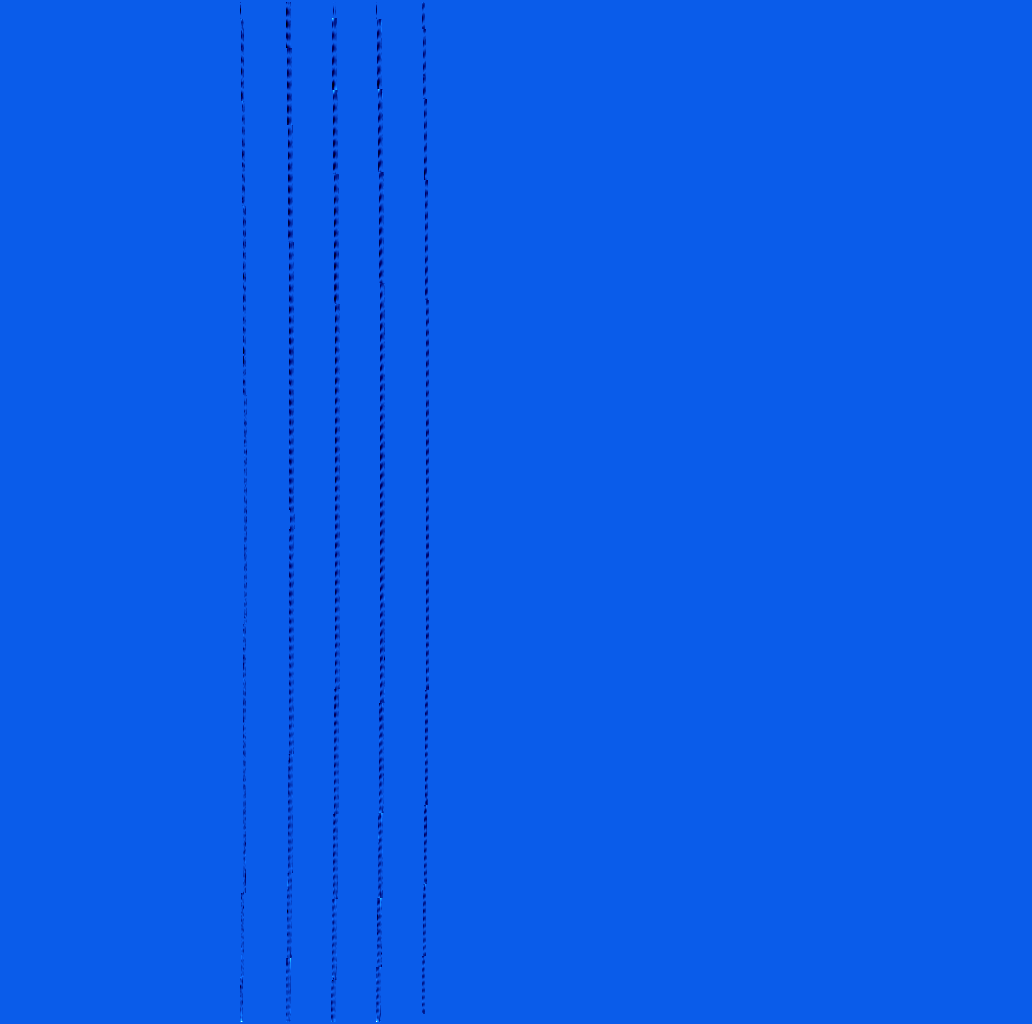
\includegraphics[width=5.5cm]{FM_ptsource_flat.png}
	\caption{Fringe flat derived from FM data for a point source in channel 1A at $\alpha=1.001$, $\beta=0.602$. Color scale is linear.}
	\label{fig:ptsrcfringeflat}
\end{wrapfigure}
Ultimately the data collection from the FM campaign produced a series of fringe flats of an almost point like at various position across the detector and in each channel.
We implemented a new routine into the \verb|pySpecSim| module of MIRISIM to read in the location of point sources within a scene, and apply the nearest available position dependent fringe flat. 
Dithered observations are accounted for, with unique fringe flats being applied to each exposure.
A new dithering strategy was designed, such that the locations of each exposure correspond to the locations of the nearest fringe flat to the standard dither offsets.

This implementation comes with several caveats: namely that the fringing model is not yet fully developed, so it can only be considered accurate for point sources located at the same ($\alpha,\beta$) location as the source used to produce the fringe flat. Additionally, the source used to generate the data is not a true point source, nor are there fringe flats produced for the full MRS wavelength range.
We stress that the goal of this testing is to demonstrate the significance of this effect to justify the need for a more complete model along with additional calibration data to constrain the detector layer parameters.

\section{JWST Pipeline}
The JWST Pipeline is used for reducing all data from the telescope, and is currently under development by the Space Telescope Science Institute. The latest version of the pipeline (v0.15a) is used for all processing within this work \parencite{Bushouse2015}.
It is broken into several stages. 
Stage one is applied to all telescope data, and corrects for detector level effects.
Stage two provides photometric calibration, with separate pipelines for imaging or spectroscopic data.
Stage three, which is unusued in this work, will provide high level science products for end users.%JWST Pipeline
 % MIRI MRS Cal pipeline
\subsection{Stage 1 Processing}
The raw data files read from MIRISIM (or eventually the MIRI instrument itself) are a series of \textit{exposures}, each made up of set of \textit{integrations} containing a some number of \textit{groups} or frames.
Each group is a non-destructive readout of the detector arrays, providing a series of increasing counts known as ramps in DN (digital number per second). 
The first stage of the JWST pipeline takes these raw files, applies a series of steps and outputs a single file for each input exposure in units of countrate.
During this stage, several data quality checks are performed, looking for saturated pixels or jumps in in the data, which can be used to correct for cosmic rays.
Dark current correction is also applied.
Finally, the set of frames in an integration are fit with a linear slope in order to calculate the count rate in DN/s.
This procedure is applied to all MIRI data.
We used default pipeline settings to apply this procedure, and applied all steps applicable to the MIRI instrument.
The particular calibration procedures for MIRI MRS data is described in \parencite{ref:mirical}.
\subsection{Stage 2 Processing}
For the second stage of processing we use the Stage 2 Spectroscopic Processing pipeline, and apply the steps individually to maintain control over parameters.
The second stage pipeline applies instrument specific corrections that result in a photometrically calibrated exposure. For the MRS, this involves the following series of steps, some of which will be described in further detail below.
\begin{enumerate}
	\item \verb|assign_wcs| Assign a World Coordinate System (WCS) to each exposure.
	%\item \verb|background| Perform image-from-image background subtraction.
	\item \verb|flat_field| Flatten photometric variation from differences in gain and dark current.
	\item \verb|srctype| Assign whether the target is a point or extended source based on input from the raw data files or observation parameters.
	\item \verb|straylight| Remove known stray light component.
	\item \verb|fringe| Divide by an extended source fringe flat.
	\item \verb|photom| Photometrically calibrate the exposure based on known pixel sensitivities and areas.
	\item \verb|cube_build| Transform from a (set of) 2D detector images to a 3D IFU cube in ($\alpha,\beta,\lambda$).
\end{enumerate} 
\subsubsection{Photometric Calibration}
Photometric calibration is the process of removing detector and optical biases to ensure that the measured output corresponds to the true flux incident onto the telescope.
This process occurs in the PHOTOM step of the JWST pipeline, and uses reference files which store per-pixel photon-to-electron conversion efficiencies along with pixel areas in arcsec to transform the count rate data product to a surface brightness measurement.
This corrects for the wavelength dependent bias shown in Fig. \ref{fig:mirideteff}.

However, this step remains under development, and does not produce absolutely calibrated images. In particular, even using the most up to date reference files (v8D.04.00) there remains discontinuities between channels, and poorly calibrated spectral slopes.

\subsubsection{Fringing correction}
Fringing correction within the JWST pipeline is accomplished by dividing a known fringe flat into the photometrically calibrated detector image. 
This fringe flat is based of extended source CV data, and a unique flat is used for each detector/sub-band configuration.

\subsubsection{Cube Building}
In order to extract the spectrum measured by the MRS, the detector image is converted into an IFU Cube in $(\alpha,\beta,\lambda)$ space, using the transformation which was outlined in Fig. \ref{fig:mrscoords}.
A set of transformations for each band maps each detector pixel to a a spaxel in cube space, accounting for  optical distortions. 
These transformations produce an irregular grid that samples the on-sky intensity, which can then be combined into a regularly spaced grid of spaxels.
Each spaxel filled by a weighted sum of points, with the weight decreasing with distance from the spaxel. 
This should also account for changes in the MIRI PSF with wavelength, however issues with the cube building prevent use of the \verb|miripsf| weighting scheme.
Instead, the flux-conserving Shepards method is used, setting the weighting parameter to \verb|'emsm'|.
It should be noted that this procedure introduces correlations between the spaxels, which is not accounted in the error on each spaxel.

\subsubsection{Aperture Photometry}

Once the data from the pipeline has been transformed into a spectral cube, we can perform aperture photometry using the \verb|photutils| package to extract a 1D spectrum of the source.
For each frame in each sub-band the coordinates of the spaxel at with the peak flux is detected using \verb|photutils| \verb|find_peaks|, which provides the location for the center of a circular aperture.
A radius of 5 spaxels is used to encompass the entire PSF for a point source.
The input file must be photometrically calibrated, with units of surface brightness in mJy/as$^{2}$.
Using the \verb|aperture_photometry| function, we sum all of the contributions within the central aperture.
Using a set of additional apertures, we measure and subtract the median background surface brightness.
This measurement is then converted into flux units by multiplying by the spaxel area in as$^{2}$.
The standard deviation of the background measurements is used to define the error on the flux measurement.
While optimal extraction techniques exist, given our known input signal and background, this procedure is adequate for producing a spectrum in each sub-band, which can then be combined into a single spectrum for all measured sub-band.
\begin{figure}[t]
	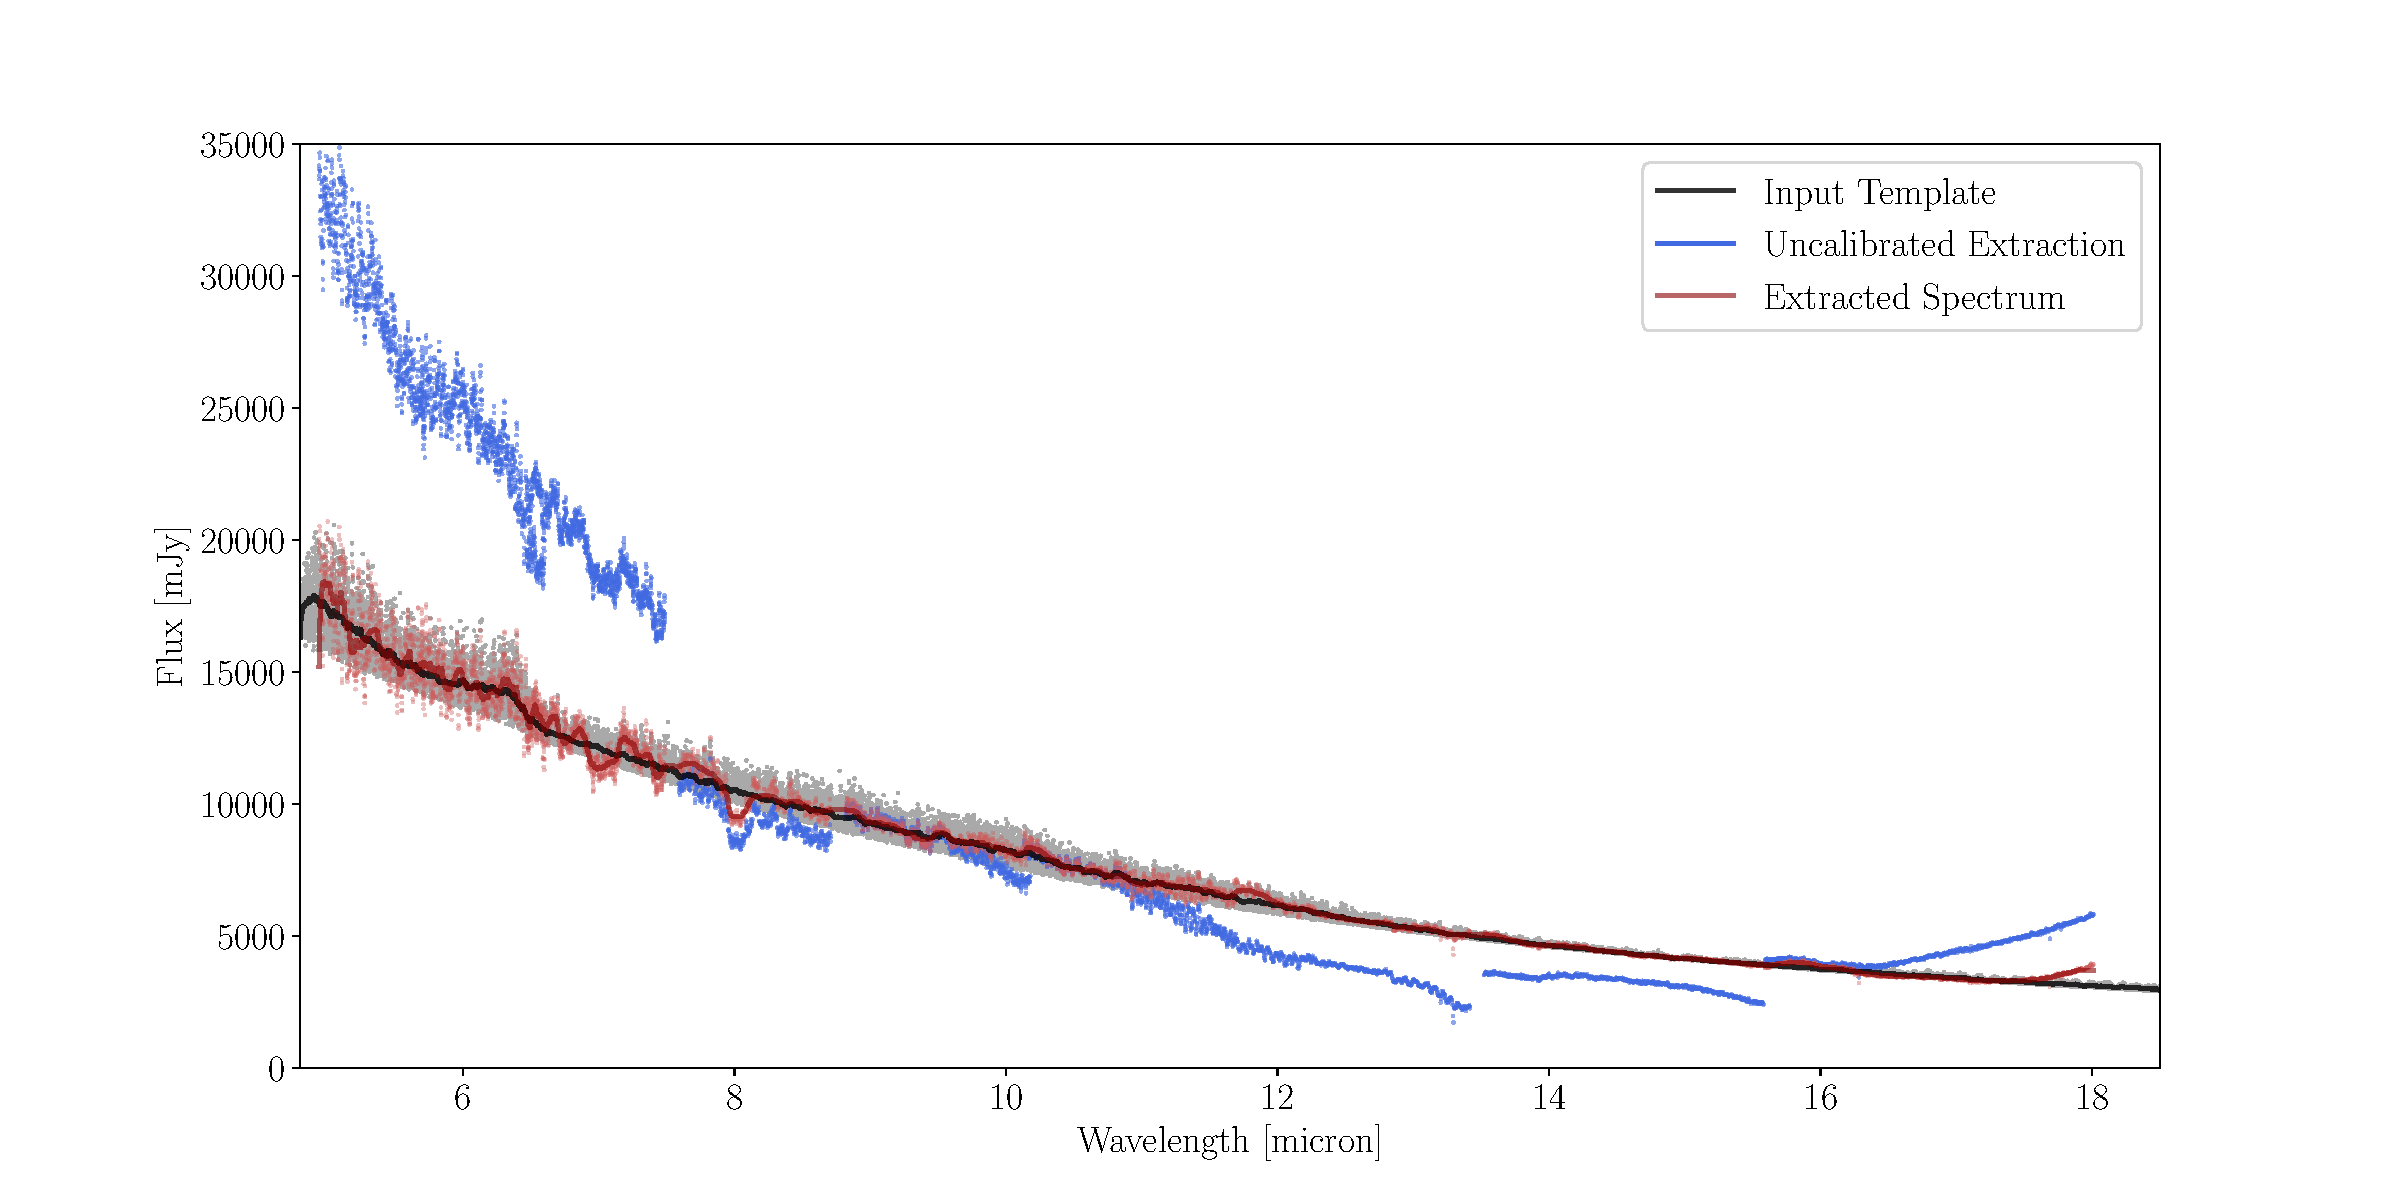
\includegraphics[width=1.11\linewidth]{cal_spectra_slope.pdf}
	\caption{Comparison of an input spectrum generated using petitRadTrans and the empirically calibrated output spectrum after extraction using aperture photometry from the cube produced by the JWST pipeline.}
	\label{fig:cal}
\end{figure}

Unfortunately, due to the issues described above with the PHOTOM step of the JWST pipeline, the spectrum built using aperture photometry does not accurately reflect the input spectrum in slope or absolute photometry. 
Therefore, we correct the extracted spectrum channel by channel. 
We fit a cubic polynomial to a median filtered copy of both the template spectrum and the extracted spectra.
The cubic fit to the extracted spectra is subtracted from the data, and the fit to the template is added. 
Thus this procedure corrects the slope and median flux value, but does not affect high frequency noise or signals.
Fig. \ref{fig:cal} shows an example of the results of this procedure. 
We believe that this is a justified measure, as the errors with photometric calibration in the pipeline should be resolved before first light of the telescope.

\section{Cross-Correlation}\label{sec:cc}
To quantify the similarity of the spectrum output by the JWST pipeline to the input into MIRISIM, we rely on the technique of cross correlation.
Originally used in a spectroscopic context by \parencite{Simkin1974} in order to compute galaxy velocity dispersions, cross correlations have become a popular technique used to quantify exoplanet parameters \parencite{Snellen2014}.

For two arbitrary, complex-valued functions $f(t)$ and $g(t)$, we can compute the cross correlation as as function of the shift $\tau$ between the functions (typically in time or velocity space):
\begin{equation}\label{eqn:crosscorr}
\left(f \star g\right)(\tau) \equiv \int_{-\infty}^{\infty}f^{*}(t)g(t + \tau)dt
\end{equation}
Our signals of interest are astrophysical spectra, measured in a finite number of discrete wavelength bins. For such a signal with $M$ bins:
\begin{equation}\label{eqn:discretecorr}
\left(f \star g\right)[n] \equiv \sum_{m=0}^{M}f^{*}[m]g[m + n]
\end{equation}

Care must be taken when cross-correlating signals, as differences in normalization can result in changes in the correlation coefficient. 
Our procedure takes in two spectra. 
The first is an emission spectrum produced by the petitRADTRANS program \parencite{Molliere2019}, which provides our forward model with which we compare our data spectrum.
Our data is the result of passing the template spectrum through MIRISIM, and extracting it from the resulting detector image using the JWST pipeline.
We then rebin the high-resolution input spectrum to the same wavelength bins as the data spectrum, using the \verb|spectres| package \parencite{Carnall2017}.
Prior to normalization, we remove any outliers from the spectrum (due to binning errors or instrumental effects) by setting any data points separater by more than 15 standard deviations from the mean to the median value of the spectrum.
For each spectrum, we subtract the minimum value to remove any offset in the spectrum, and divide by the maximum value to restrict the range to [0,1]. 
We then use apply a Savitzky-Golay filter with a window of 1/4 the length of the spectrum and a polynomial order of 3, which we then subtract from the unfiltered spectrum. 
This removes the continuum emission from the spectrum, and centers it around 0.
We then renormalize the spectrum by dividing by the maximum absolute value such that the range is in [-1,1]. 

The cross correlation between the forward model and itself is computed, excluding the region of interest around 0 offset. 
This `autocorrelation' is subtracted from the cross correlation between the forward model and the data spectrum in order to remove secondary peaks.
Finally, we normalize the cross correlation by the standard deviation of the cross correlation (excluding the central peak), giving an output measured as a signal to noise ratio.
\begin{figure}[h]
	\centering
	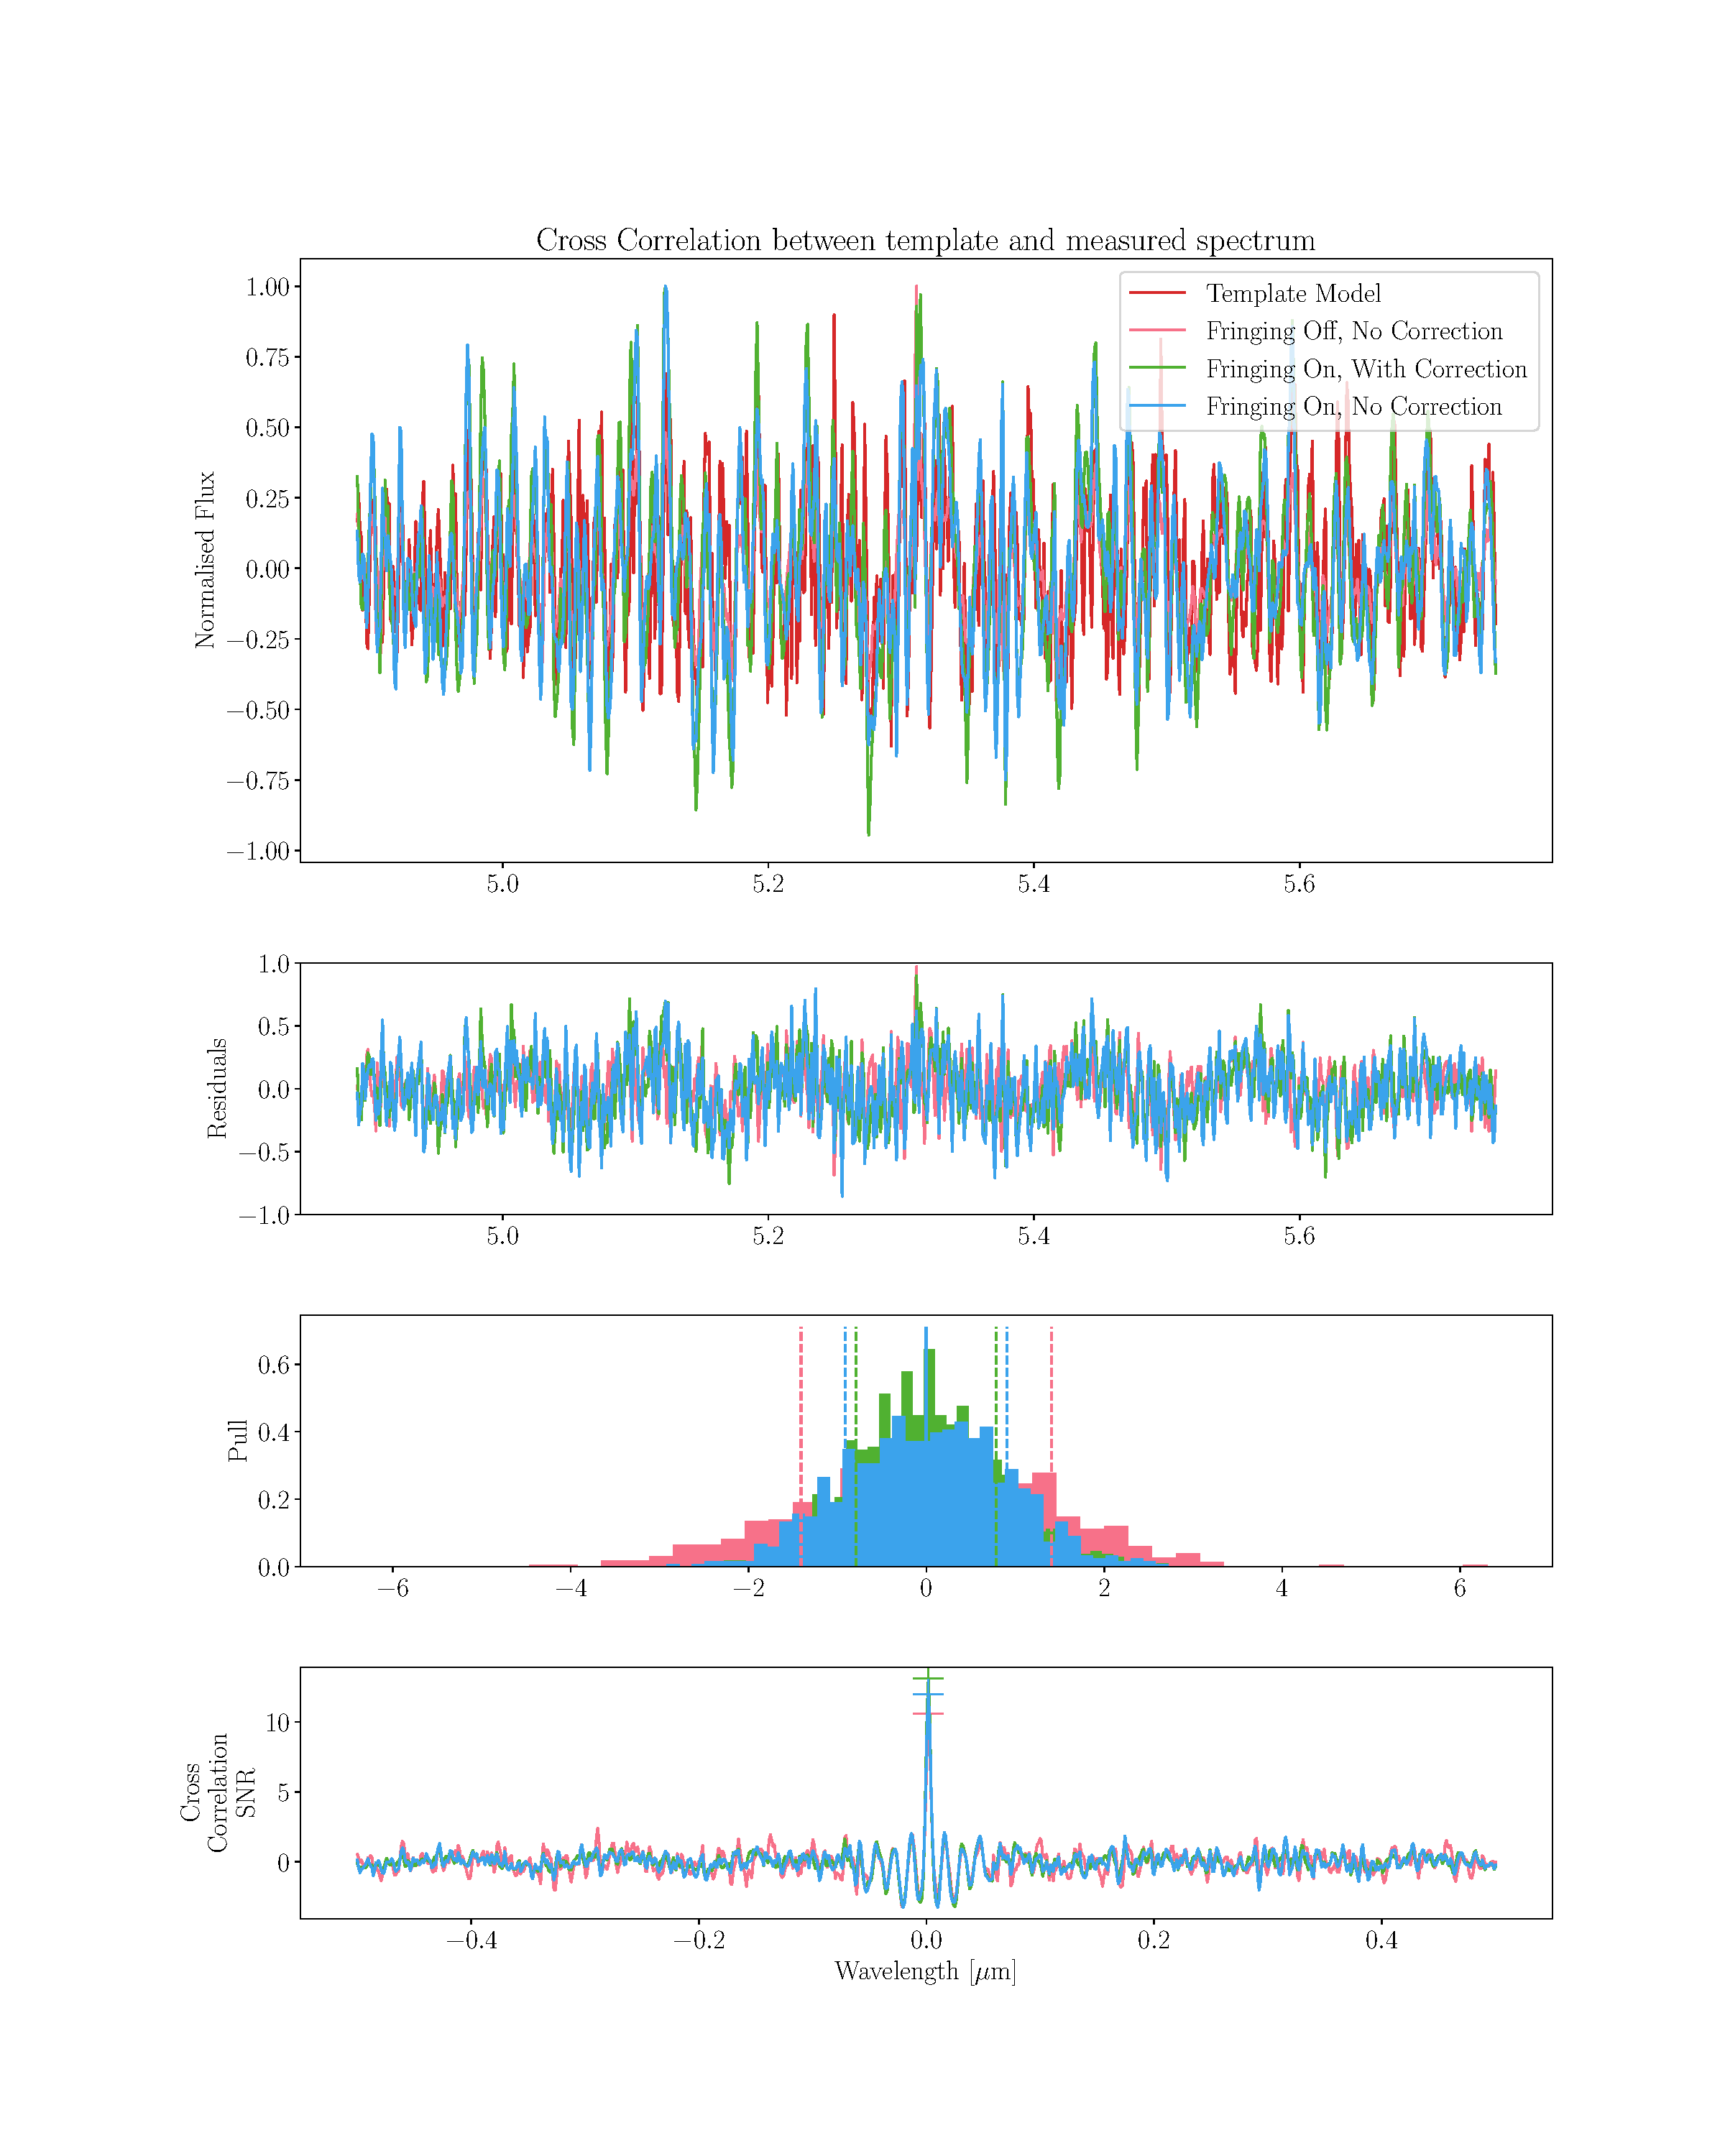
\includegraphics[width=0.9\linewidth,trim=4cm 3.5cm 4cm 4.5cm]{hr8799eclosecor_v5}
	\caption{FIXME FIXME FIXME - Use correct planet model. \textbf{A} Normalized spectra of VHS1256b, with the input template in red, a spectrum with no fringing and no correction applied in pink, with extended source fringing and with correction in green, and extended source fringing and no correction in blue. \textbf{B} Residuals found from subtracting the extracted spectra from the input template. \textbf{C} Histogram of residuals. Note the difference in the distribution widths due to fringing. \textbf{D} Cross correlation between the extracted spectra and the template.}
	\label{fig:CrossCor1D}	
\end{figure}

\subsection{Molecular Mapping}
Cross correlations are used to identify the presence of a given molecular species in the spectrum of an atmosphere \parencite{Hoeijmakers2018,Haffert2019}.
As shown above, fringing has a significant impact on cross-correlations. 
By extending our iterating over each spaxel from the MRS cube and using a molecular template rather than the input spectrum, we can examine the impact of fringing on such an analysis.
\begin{figure}[t]
	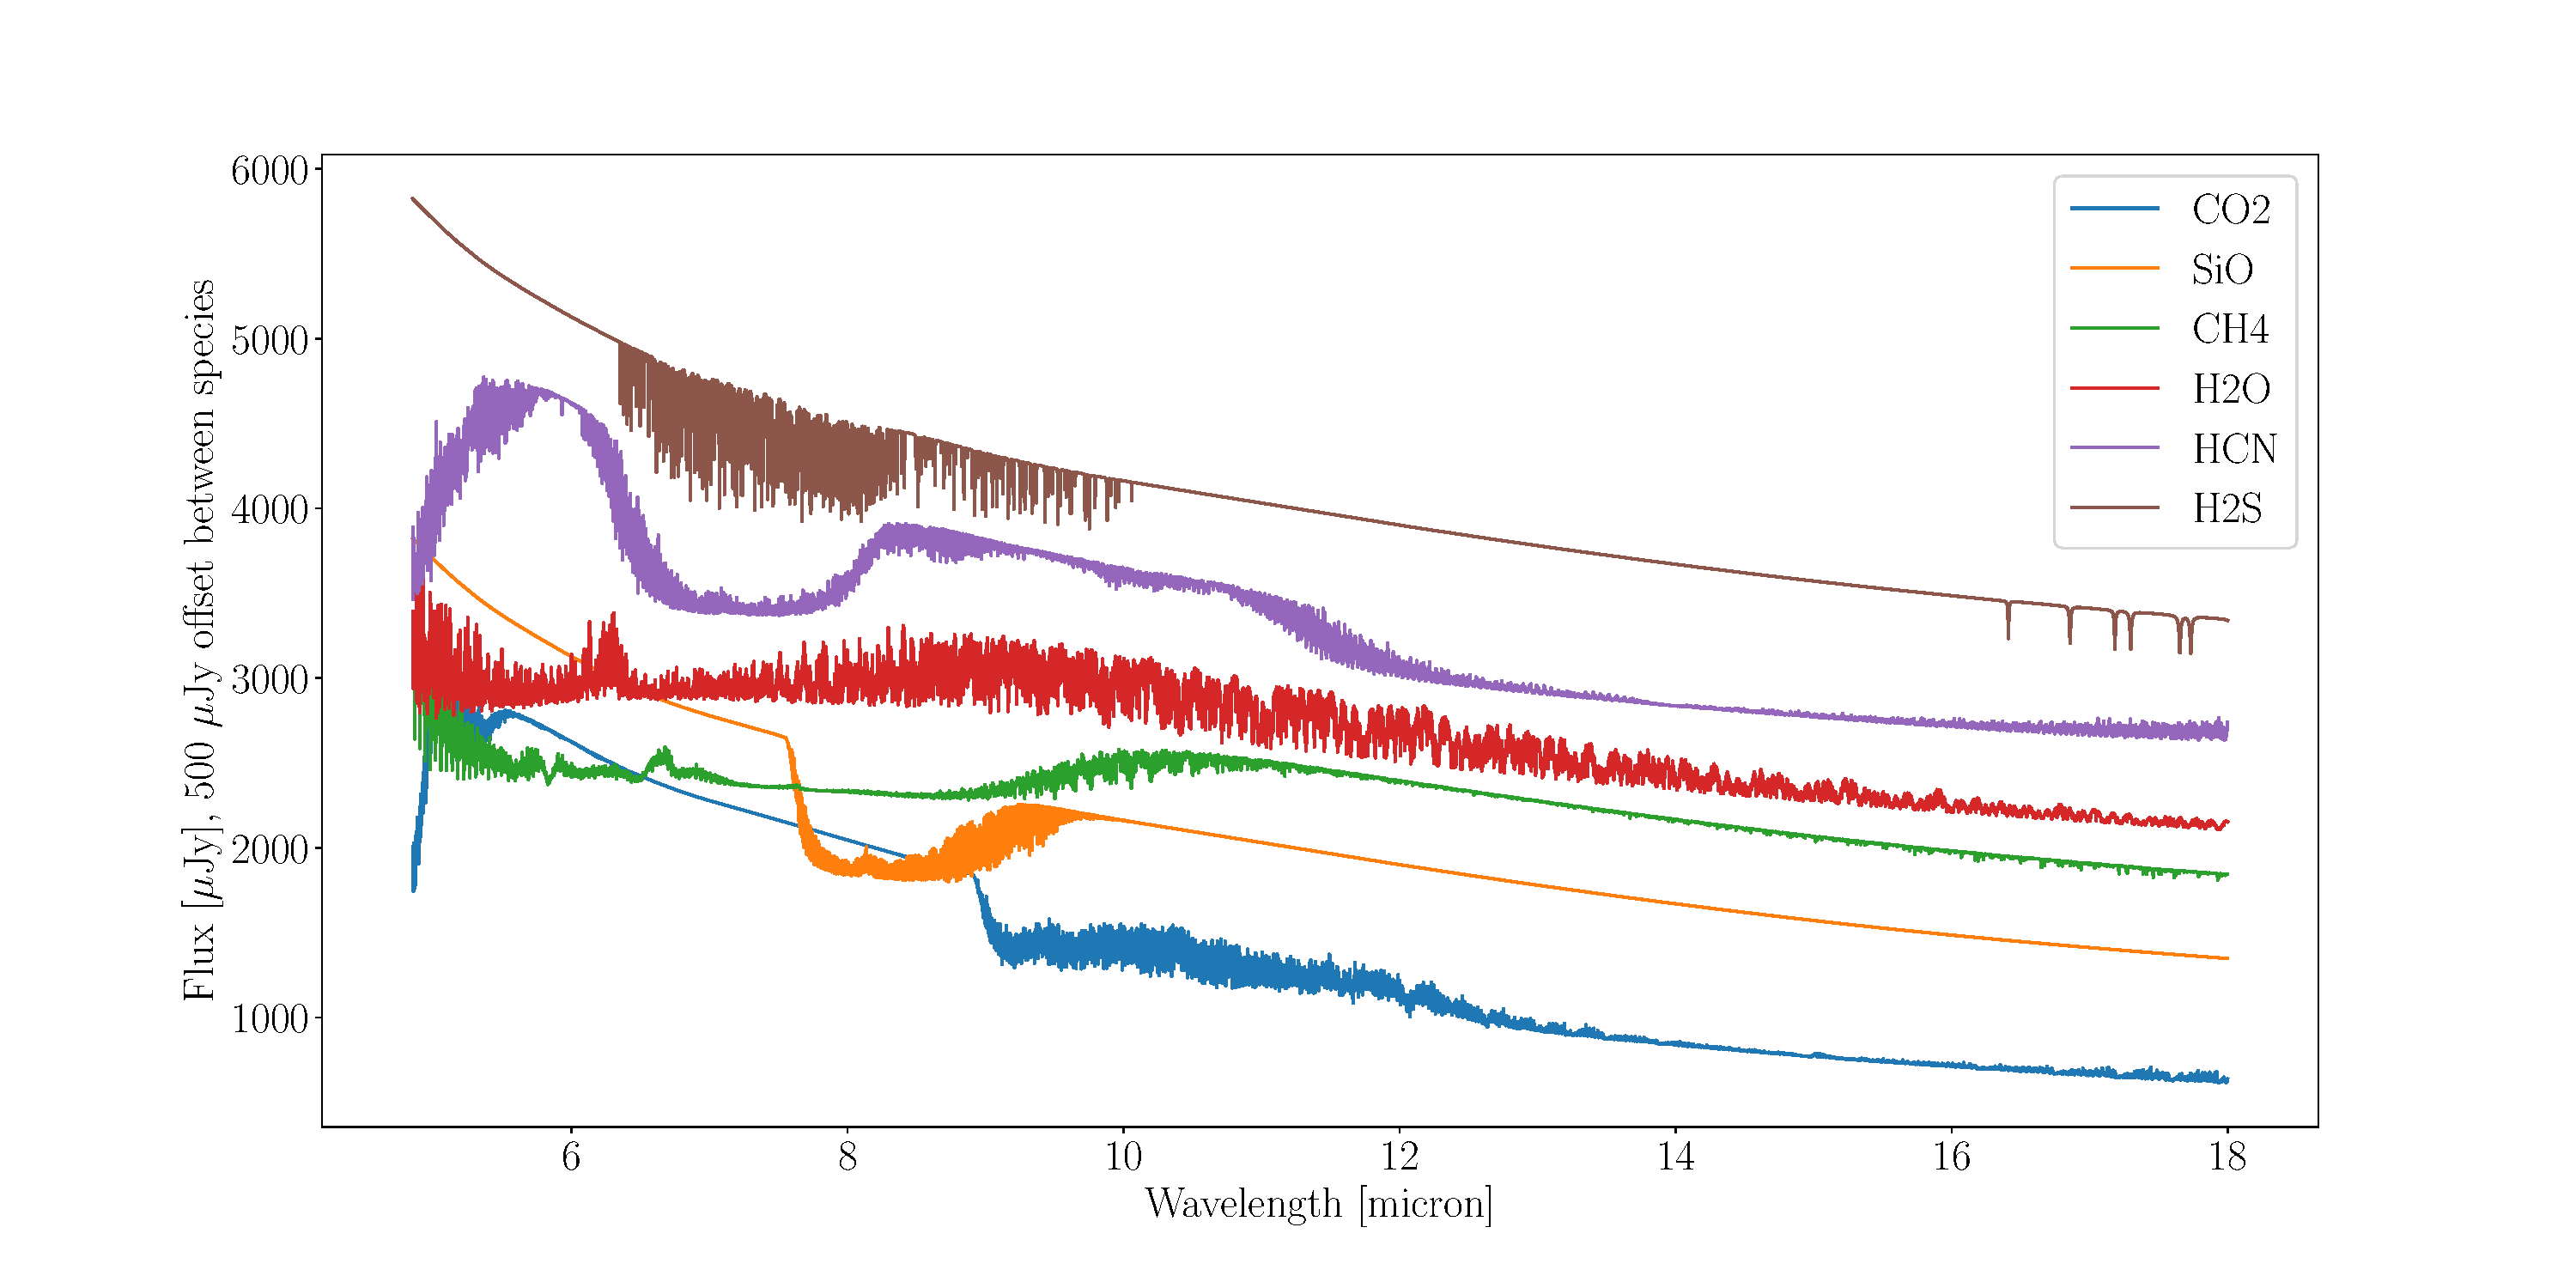
\includegraphics[width=\linewidth]{VHSSpeciesTemplates}
	\caption{Species templates for VHS1256b. Each species emission spectrum is computed using petitRADTRANS with a single species atmosphere with Jupiter-like abundances of H$_{2}$ and He, and an internal temperature of 900 K. There is a 500$\mu$Jy offset between each species.}
	\label{fig:speciestemplates}
\end{figure}

We use petitRADTRANS to generate a single-species atmosphere in order to generate the molecular emission spectrum templates. 
We chose to use VHS1256b as our template for this study, and all other atmospheric parameters remain the same, as described in table \ref{tab:petitradparams}. 
A fractional abundance of 1\% was used for each species.
The emission spectrum for each of these species is shown in Fig. \ref{fig:speciestemplates}.
Using the same normalization procedure described in section \ref{sec:cc} for each spaxel, we take the peak cross correlation value from within a narrow window around the expected peak at 0 offset between the template and measured spectra. 
This was repeated for each of the fringing cases and each of the molecular templates. 
We also compare the cross correlation as computed sub-band by sub-band to the full wavelength range used.
\begin{figure}[t]
	\centering
	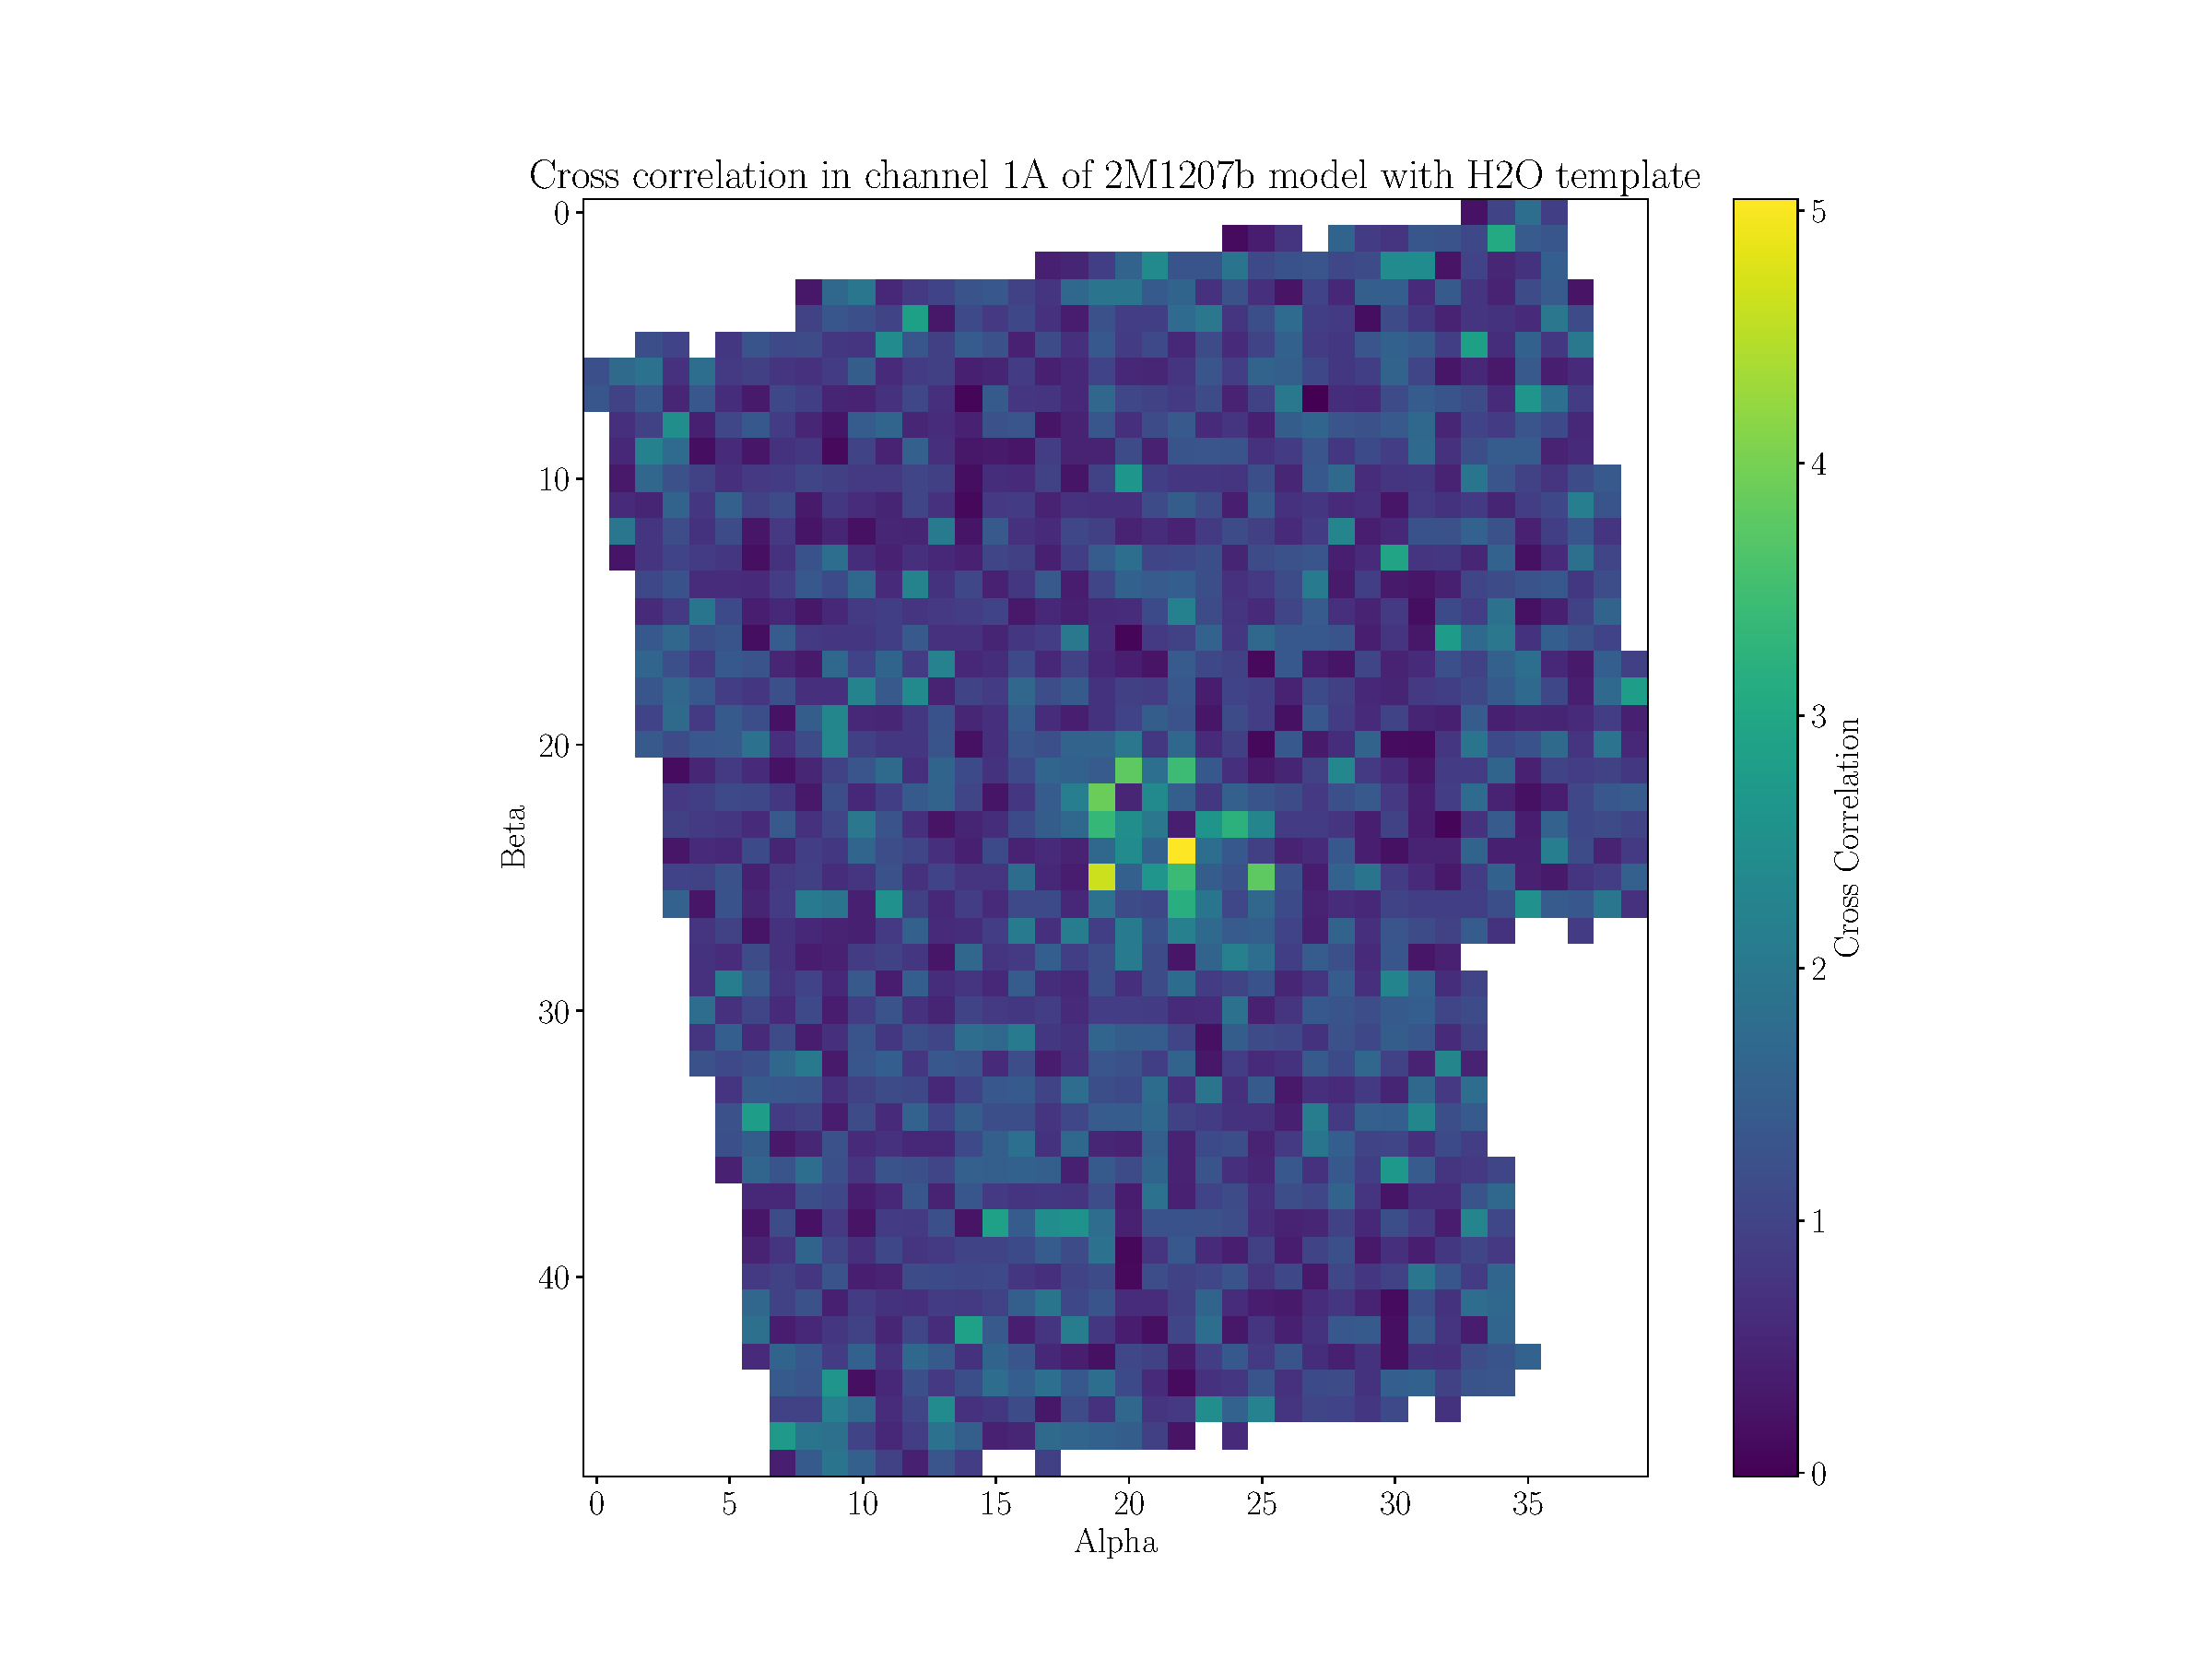
\includegraphics[width=0.8\linewidth]{IFU_CrossCor_Test}
	\caption{Pixel by pixel cross correlation between the extracted 2M1207b spectrum with an H2O template spectrum. FIXME FIXME FIXME add with/without fringing.}
	\label{fig:h2omap}
\end{figure}
\clearpage
\section{Results}
%\begin{table}[h]
%	\begin{tabular}{cr|c|c|c|c|}
%		\toprule
%		&& \multicolumn{4}{c}{MIRISIM Fringing Model}\\
%		&& None & FM Extended & FM Point On Axis & FM Point Off Axis\\
%		\midrule
%		\parbox[t]{2mm}{\multirow{2}{*}{\rotatebox[origin=c]{90}{Correction}}}  & None & & & &\\[50pt]
%		& Ext. Flat  & & & &\\[50pt]
%		\bottomrule
%	\end{tabular}
%\end{table}

\subsection{Residual Statistics}
In addition to computing the cross correlation between the forward model and the data spectrum, we also examine the residuals between the two spectra.
Here we can see any unexpected variations between the two (periodic signals, offsets or other features).
We can also examine a histogram of the residuals, normalized by the standard deviation of the data spectrum.
This provides us with a  distribution which should have a mean of 0 and unit width if the data are unbiased and share a distribution with the true input spectrum.

\subsection{Fringing Results}
1. A stronger input signal results in a stronger correlation.

2. Fringing does NOT necessarily degrade the cross correlation SNR, but rather increases it. The scale of this increase seems to depend on the absolute magnitude of the correlation (ie, a larger increase at higher SNR)

3. The residuals from subtracting the template from the data has structure.

4. If the residuals are histogrammed (and normalized by the standard deviation of the data), the width of the distribution may correspond to the cross correlation SNR (wider distribution = lower SNR)

5. Only when strongly increasing the fringing effect does the SNR decrease.

6. Correcting for fringing using the standard JWST fringe map decreases the SNR when compared to the case of fringing with no correction, but is typically still above the no-fringing case.

7. The JWST correction performs worse in the off axis case, as the fringe pattern begins to vary more when compared to the CV fringing model.

\subsection{Fringing Correction}
1. Extended Flat Correction on Extended Flat Input

2. Extended Flat Correction on Point Source input

3. Iterative Correction on Extended Flat Input

4. Iterative Corretion on Point Source input

